% !TEX root = ../thesis.tex
%
\chapter{System Design}
\label{ch:design}

...

At the time of beginning the implementation, the current Elasticsearch and Kibana versions were 6.1.1, the current Event Store version was 4.1.

\section{Assumptions}
\label{sec:design:assumptions}

Certain assumptions and restrictions are made in order to limit the complexity of \acf{IFAS} without reducing the results' significance.

\begin{description}
\item[HTML \& JS Client] The client application which is used for generating data for testing and evaluation purposes will be a web application using \ac{HTML} and JavaScript.
This choice is influenced by personal preference, but is backed by research on experimentation~\cite{Dmitriev2017,Kohavi2013a} and implicit user feedback~\cite{Joachims2005,Huang2011} also specifically targeting web applications.
As the data is sent via \ac{HTTP}, the passive user feedback could in theory also be implemented in any other programming language which supports sending of \ac{HTTP} requests, such as Java or C\#.
\item [...]
\end{description}

\section{Goals}
\label{sec:design:goals}

\begin{enumerate}
\item A web application sends passive user feedback data to specifiable streams of the Event Store instance.
The type of application is not important, but should be geared toward typical end users (instead of a business application).
Instead of implementing an application from scratch, an existing open source application shall be modified to send this data in order to save the additional time for creating the application.
The reasons why a web application is used as a data source, and not, as initially planned, the Rico data set, are explained in the following \cref{sec:design:data-source}
\item The usability of the web application can be evaluated via some metrics, which have to be created in the process.\todo{read up on UX testing, specify further}
\item Elasticsearch is fed with all events that are created while users interact with the application.
It can be specified which streams this data shall come from, as it is plausible that other data is saved to the event store.
\item The collected user feedback can be analyzed via Kibana.
For this purpose, one or more graphical representations of the usability metrics are created.
\item The passive feedback system can be deployed on any machine which supports Docker, i.e. Windows, Linux and MacOS.
\item User feedback can be accessed within Kibana within a few seconds from occurrence of the user action; at the absolute most this may take half a minute (30s).
This is to allow for fast reactions to critical \ac{UX} errors such as a button invoking a critical action becoming unavailable.
\end{enumerate}


\section{Choosing a User Data Source}
\label{sec:design:data-source}
% why the RICO data set was not used

Die Interaction Traces versprechen, dass alle UIs der Apps dort hinterlegt sind, in der Realitaet haben die Nutzer und/oder der Crawler aber oft total komische Aktionen ausgefuehrt oder sind nicht ueber das Setup der App hinaus gekommen (stichpunktartige Ueberpruefung der Daten).
Dadurch sind sowohl die Interaction Traces als auch die UI-Daten ansich oft nicht "richtig".
Ausserdem existiert oft nur 1, ansonsten meist nur 2, Interaction Traces.

Fazit: Leider unbrauchbar!
Alternative: bestehende Applikation um *Listener* erweitern. Literatur von Kohavi et al lesen um Hinweise zu erhalten wie man das implementieren kann

Instead, it was decided that an existing web application shall be modified such that it sends passive user feedback via \ac{HTTP} to the event store.
This application is the cloud-based messaging application Mattermost\footnote{\url{https://about.mattermost.com/}}.
As the Mattermost server as well as the client application is open source and offers the possibility to be hosted on a private server, it fits the requirements for the data source listed in \cref{sec:design:goals}.
Apart from that, this decision was at least partly based on personal preference due to familiarity with Mattermost and the web application being implemented in React\footnote{\url{https://reactjs.org/}}.

\section{Metrics Selection}
\label{sec:design:metrics}

WIP
\cite{Kelly:2003:IFI:959258.959260}
\cite{Claypool2001}

% Identifying the metrics to evaluate created customer value and product success was a challenge both in relation to dedicated experiments and to the general observation of product usage \cite{lindgren2015software}

\citet{Kohavi2013a} stress the importance of defining an \ac{OEC} which distills important metrics such as revenue or customer satisfaction in one single metric.
Having a fitting \ac{OEC} eliminates the need to carefully balance out the other metrics, as they are represented by the \ac{OEC}.
\citeauthor{Kohavi2013a} give an example where market share is a bad \ac{OEC} for a search engine, as worsening the search algorithm would increase the amount of search queries in the short term and thus increase market share; in the long run, users would use an alternative product and thus this \ac{OEC} would drop again.
Sessions per user would be a much better \ac{OEC} in this example, \citeauthor{Kohavi2013a} say.

\section{Event Structure}
\label{sec:design:event-structure}

Regardless of the specific event type, some attributes are always of interest and therefore included in every event; this is the \texttt{GenericEvent} interface in \cref{fig:event-structure}.
These attributes are:

\begin{description}
\item[@timestamp] The time at which the event occurred; the @ prefix is given in order to have Elasticsearch automatically detect this as the timestamp.
\item[EventType] This denotes the event type; maps to the \texttt{EventType} of the event in the event store.
\item[Data] This field contains the event's contents, which depend on the event type.
\item[User] Anonymized user data is added to the event, such that it is possible to recreate an interaction trace of the given user, if needed.
\end{description}

There are X different event types, which inherit the event structure from \texttt{GenericEvent} and provide different data.
The event types are \texttt{UserClicked}, \texttt{MessageSent}, ... and \texttt{PostCreated} (WIP).

\texttt{UserClicked} events are used to capture all clicks that a user performs in the application.
The intention is that for any application, these events give an analyst enough information to identify what the user was doing at that point.
The \texttt{UserClicked} event contains information about the clicked element such as the HTML attributes \texttt{class} and \texttt{id} as well as its inner text.
There may still be cases where this is not enough to identify the action that the user performed, which is why the event is amended with the click's position within the application, the window's height and width, and the current URL.
Using this information, the analyst can exactly identify the position where the user clicked at the given point in time.

Parts of this data may be redundant and/or unspecific in some cases, but helps to recreate the user's steps if this is needed.
The specificity of these events can be improved by assigning unique ids to every element - or at least to the ones which are of special interest.

\section{Event Store-Elasticsearch Bridge}
\label{sec:design:bridge}

In order to move the event data to Elasticsearch and afterwards into Kibana, a service is needed which bypasses the lack of a direct integration of Event Store and Elasticsearch.
This service is the Event Store-Elasticsearch Bridge (short just "bridge" in this context).

%\subsection{The Need for a Bridge Service}

Intuitively, it seems problematic that Event Store and Elasticsearch have different concepts of storing their data.
On the one hand, in Event Store, data is stored as events in streams; each event always has an event type and a distinct number within that stream.
On the other hand, in Elasticsearch, data is managed in indices which contain documents; each Elasticsearch document is assigned a document type.
These two concepts can be assigned 1:1 to each other -- each stream maps to an index, each event type maps to a document type within its respective index, and each event maps to a document (cf. \cref{table:design:bridge}).
Thus, for every event that is posted to the store, a new document of the same type shall be created in the index of the same name as the Event Store's stream.
A delay of a few seconds between the arrival of the event and its posting to Elasticsearch is acceptable.

\begin{table}[]
\centering
\caption{Mapping of Event Store to Elasticsearch data types}
\label{table:design:bridge}
\begin{tabular}{l|l}
\textbf{Event Store} & \textbf{Elasticsearch} \\ \cline{1-2}
Stream & Index \\
Event Type & Document Type \\
Event & Document
\end{tabular}
\end{table}

One possible and seemingly convenient solution would be using Logstash\footnote{\url{https://www.elastic.co/products/logstash}} as the bridge; this is not applicable in this exact scenario though.
Logstash is another application from the Elastic stack; it serves the exact purpose to integrate data from various sources into Elasticsearch.
It is possible to consume Atom feeds via Logstash's \ac{RSS} plugin, which Event Store offers an interface for.
This is not feasible for this scenario as Logstash's \ac{RSS} plugin is not able to handle feeds which require authentication, which Event Store does.
Also, Event Store's persistent subscriptions are not compatible with Atom feeds, which is another reason to abandon Logstash as a possible solution.

Instead of using an existing service that listens to Atom feeds such as Logstash, a custom implementation is the better approach here.
This is the case because the official .NET Core Event Store client \ac{API}\footnote{\url{https://github.com/EventStore/ClientAPI.NetCore}} can be used, which allows amongst others for usage of persistent subscriptions and more efficient communication over a dedicated protocol built on top of \ac{TCP}.
The \ac{TCP} protocol variant is faster than the alternative via Atom feeds, which is built on top of \ac{HTTP}\cite{WEB:EvtSt-Which-Api}.
It should be noted that, although using \ac{TCP} instead of \ac{HTTP} contradicts the requirement for an \ac{HTTP} interface as stated in \cref{sec:design:goals}, this is not a problem at all due to the technology heterogeneity that a microservice architecture allows\cite[Key Benefits,pp.~4f]{newman2015building}.

Assuming the Event Store stream already exists, setting up the bridge to transfer new events to an Elasticsearch index would then be a two-step process.
First, a persistent subscription has to be created within the Event Store administration overlay.
Then, an instance of the bridge service has to be started, configured to listen to the newly created subscription.
This would cause the bridge to transfer all existing events to an Elasticsearch index of the same name as the stream, and then also posting all subsequent events to this index.

It would also be possible to implement the bridge in a way that allows the service to listen to multiple subscriptions simultaneously.
This would require a more complex service which introduces two problems.
First, it introduces an unnecessary implementation overhead, and second, its additional complexity could lead to scaling problems.
Writing complex, large serices is in general discouraged to do in a microservice architecture\cite[Key Benefits,pp.~5f]{newman2015building}.
Instead, multiple instances of the same service should be executed alongside each other, with their respective configuration for listening to a specific stream.

Thanks to persistent subscriptions, it is possible to temporarily take the bridge instance offline -- as the subscription state is persisted on the server side, the bridge can transfer all events that occurred while it was offline as soon as it comes online again.
Multiple instances of the bridge may listen to the same persistent subscription if heavy load is expected on the system -- this is known as the \emph{competing consumers} messaging pattern\cite{WEB:Microsoft-Competing-Consumers}.
This advanced use case is not considered further though.

\subsection{Mapping Event Store Rebuilds to Elasticsearch}
\label{subsec:design:bridge:mapping}

Problem: Elasticsearch does not support Complete Rebuild and its variants (temporal query, event replay, reversing events, delayed application(?)).
Solution: Delete index and then set up a new subscription.
The downside is that this renders the analytics application practically useless for the time span until the Elasticsearch index is repopulated with the Event Store data.
Some implementation details regarding this problem can be found in \cref{subsec:implementation:bridge:mapping}

\section{Final Architecture}

\begin{figure}[htb]
        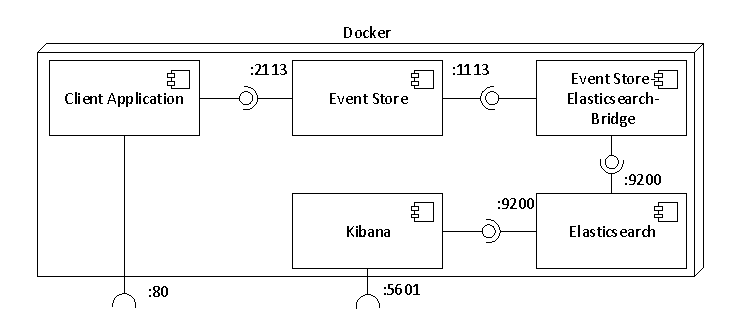
\includegraphics[width=\textwidth]{gfx/docker-architecture}
        \caption{}
        \label{}
\end{figure}





































